\hypertarget{pf__administration_8h}{
\section{pf\_\-administration.h File Reference}
\label{pf__administration_8h}\index{pf\_\-administration.h@{pf\_\-administration.h}}
}


This graph shows which files directly or indirectly include this file:\nopagebreak
\begin{figure}[H]
\begin{center}
\leavevmode
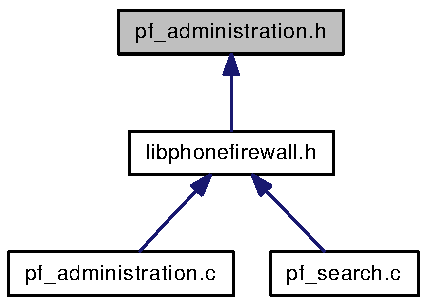
\includegraphics[width=120pt]{pf__administration_8h__dep__incl}
\end{center}
\end{figure}
\subsection*{Functions}
\begin{CompactItemize}
\item 
int \hyperlink{pf__administration_8h_6c03680796f887d3851428fb2b9ecbc5}{add\_\-entry} (int country\_\-code, int area\_\-code, unsigned long long number, char $\ast$name, char $\ast$reason, int priority, int listflag)
\item 
int \hyperlink{pf__administration_8h_b6c4b54e76914072e8c0d06f9e450d33}{rm\_\-entry} (int country\_\-code, int area\_\-code, unsigned long long number, int listlfag)
\item 
int \hyperlink{pf__administration_8h_754e9a8891128a285fc17132b5480a07}{check\_\-entry} (int country\_\-code, int area\_\-code, unsigned long long number, int priority, int listflag)
\item 
int \hyperlink{pf__administration_8h_2edf8cd83efaa23984150c5c7e62d628}{check\_\-entry\_\-string} (char $\ast$number, int priority, int listflag)
\item 
int \hyperlink{pf__administration_8h_a3f4effcf850afd9ac912fe3ec7c7b16}{change\_\-name} (int country\_\-code, int area\_\-code, unsigned long long number, char $\ast$new\_\-name, int listflag)
\item 
int \hyperlink{pf__administration_8h_2dff06b890556fd5ac9f992c925d5550}{change\_\-number} (int country\_\-code, int area\_\-code, unsigned long long number, int new\_\-country\_\-code, int new\_\-area\_\-code, unsigned long long new\_\-number, int listflag)
\item 
int \hyperlink{pf__administration_8h_f57945a657640ebf2333991484bd8a4c}{change\_\-reason} (int country\_\-code, int area\_\-code, unsigned long long number, char $\ast$new\_\-reason, int listflag)
\item 
int \hyperlink{pf__administration_8h_985dd7c968f457400d40538864fee0c0}{change\_\-priority} (int country\_\-code, int area\_\-code, unsigned long long number, int new\_\-priority, int listflag)
\end{CompactItemize}


\subsection{Function Documentation}
\hypertarget{pf__administration_8h_6c03680796f887d3851428fb2b9ecbc5}{
\index{pf\_\-administration.h@{pf\_\-administration.h}!add\_\-entry@{add\_\-entry}}
\index{add\_\-entry@{add\_\-entry}!pf_administration.h@{pf\_\-administration.h}}
\subsubsection{\setlength{\rightskip}{0pt plus 5cm}int add\_\-entry (int {\em country\_\-code}, int {\em area\_\-code}, unsigned long long {\em number}, char $\ast$ {\em name}, char $\ast$ {\em reason}, int {\em priority}, int {\em listflag})}}
\label{pf__administration_8h_6c03680796f887d3851428fb2b9ecbc5}


Add a number to the blacklist/whitelist. The number will be blocked after that.

\begin{Desc}
\item[Parameters:]
\begin{description}
\item[{\em country\_\-code}]The country code (for example 39 for Italy, 43 for Austria, and so one) \item[{\em area\_\-code}]The area code which indicates your mobile operator. \item[{\em number}]The telephone number of the person (without country and area code. \item[{\em name}]The name of the person. \item[{\em reason}]Why you have blocked this person. \item[{\em priority}]Gives the \hyperlink{structentry}{entry} a priority. 0 is standard. If the priority is higher the value will be also blocked/accepted if a higher priority is choosen. \item[{\em listflag}]A flag, which indicates if you would use the blacklist (BLACKLIST\_\-FLAG) or the whitelist (WHITELIST\_\-FLAG).\par
\end{description}
\end{Desc}
The value \char`\"{}PRIO\_\-ALL\char`\"{} stands for all priorities.

\begin{Desc}
\item[Returns:]If all goes well 0 (zero) otherwise -1 and the errno variable will be set.. \end{Desc}


Definition at line 110 of file pf\_\-administration.c.

References DB\_\-FILE, ERR\_\-LOG, MAX\_\-LINE\_\-LENGTH, PRIO\_\-ALL, STMT\_\-SIZE, TB\_\-AREACODE, TB\_\-COUNTRYCODE, TB\_\-NAME, TB\_\-NUMBER, TB\_\-PRIORITY, TB\_\-REASON, and WHITELIST\_\-FLAG.\hypertarget{pf__administration_8h_a3f4effcf850afd9ac912fe3ec7c7b16}{
\index{pf\_\-administration.h@{pf\_\-administration.h}!change\_\-name@{change\_\-name}}
\index{change\_\-name@{change\_\-name}!pf_administration.h@{pf\_\-administration.h}}
\subsubsection{\setlength{\rightskip}{0pt plus 5cm}int change\_\-name (int {\em country\_\-code}, int {\em area\_\-code}, unsigned long long {\em number}, char $\ast$ {\em new\_\-name}, int {\em listflag})}}
\label{pf__administration_8h_a3f4effcf850afd9ac912fe3ec7c7b16}


Changes the name of the \hyperlink{structentry}{entry}. For the unique identification you need to enter the country code, area code and the number because this tripple identifies the \hyperlink{structentry}{entry}.

\begin{Desc}
\item[Parameters:]
\begin{description}
\item[{\em country\_\-code}]The country code (for example 39 for Italy, 43 for Austria, and so one) \item[{\em area\_\-code}]The area code which indicates your mobile operator. \item[{\em number}]The telephone number of the person (without country and area code. \item[{\em new\_\-name}]The new name \item[{\em listflag}]A flag, which indicates if you would use the blacklist (BLACKLIST\_\-FLAG) or the whitelist (WHITELIST\_\-FLAG).\par
\end{description}
\end{Desc}
\begin{Desc}
\item[Returns:]If the number was changed 1, otherwise 0. \end{Desc}


Definition at line 326 of file pf\_\-administration.c.

References DB\_\-FILE, ERR\_\-LOG, MAX\_\-LINE\_\-LENGTH, STMT\_\-SIZE, TB\_\-AREACODE, TB\_\-COUNTRYCODE, TB\_\-NAME, TB\_\-NUMBER, and WHITELIST\_\-FLAG.\hypertarget{pf__administration_8h_2dff06b890556fd5ac9f992c925d5550}{
\index{pf\_\-administration.h@{pf\_\-administration.h}!change\_\-number@{change\_\-number}}
\index{change\_\-number@{change\_\-number}!pf_administration.h@{pf\_\-administration.h}}
\subsubsection{\setlength{\rightskip}{0pt plus 5cm}int change\_\-number (int {\em country\_\-code}, int {\em area\_\-code}, unsigned long long {\em number}, int {\em new\_\-country\_\-code}, int {\em new\_\-area\_\-code}, unsigned long long {\em new\_\-number}, int {\em listflag})}}
\label{pf__administration_8h_2dff06b890556fd5ac9f992c925d5550}


Changes the number of the \hyperlink{structentry}{entry}. You need to enter the country code, area code and the number because this tripple identifies the \hyperlink{structentry}{entry}.

\begin{Desc}
\item[Parameters:]
\begin{description}
\item[{\em country\_\-code}]The country code (for example 39 for Italy, 43 for Austria, and so one) \item[{\em area\_\-code}]The area code which indicates your mobile operator. \item[{\em number}]The telephone number of the person (without country and area code. \item[{\em new\_\-country\_\-code}]The new country code. \item[{\em new\_\-area\_\-code}]The new area code. \item[{\em new\_\-number}]The new number. \item[{\em listflag}]A flag, which indicates if you would use the blacklist (BLACKLIST\_\-FLAG) or the whitelist (WHITELIST\_\-FLAG).\par
\end{description}
\end{Desc}
\begin{Desc}
\item[Returns:]If the number was changed 1, otherwise 0. \end{Desc}


Definition at line 365 of file pf\_\-administration.c.

References DB\_\-FILE, ERR\_\-LOG, MAX\_\-LINE\_\-LENGTH, STMT\_\-SIZE, TB\_\-AREACODE, TB\_\-COUNTRYCODE, TB\_\-NUMBER, and WHITELIST\_\-FLAG.\hypertarget{pf__administration_8h_985dd7c968f457400d40538864fee0c0}{
\index{pf\_\-administration.h@{pf\_\-administration.h}!change\_\-priority@{change\_\-priority}}
\index{change\_\-priority@{change\_\-priority}!pf_administration.h@{pf\_\-administration.h}}
\subsubsection{\setlength{\rightskip}{0pt plus 5cm}int change\_\-priority (int {\em country\_\-code}, int {\em area\_\-code}, unsigned long long {\em number}, int {\em new\_\-priority}, int {\em listflag})}}
\label{pf__administration_8h_985dd7c968f457400d40538864fee0c0}


Changes the priority of the \hyperlink{structentry}{entry}. For the unique identification you need to enter the country code, area code and the number because this tripple identifies the \hyperlink{structentry}{entry}.

\begin{Desc}
\item[Parameters:]
\begin{description}
\item[{\em country\_\-code}]The country code (for example 39 for Italy, 43 for Austria, and so one) \item[{\em area\_\-code}]The area code which indicates your mobile operator. \item[{\em number}]The telephone number of the person (without country and area code. \item[{\em new\_\-priority}]The new priority. \item[{\em listflag}]A flag, which indicates if you would use the blacklist (BLACKLIST\_\-FLAG) or the whitelist (WHITELIST\_\-FLAG).\par
\end{description}
\end{Desc}
\begin{Desc}
\item[Returns:]If the number was changed 1, otherwise 0. \end{Desc}


Definition at line 445 of file pf\_\-administration.c.

References DB\_\-FILE, ERR\_\-LOG, MAX\_\-LINE\_\-LENGTH, STMT\_\-SIZE, TB\_\-AREACODE, TB\_\-COUNTRYCODE, TB\_\-NUMBER, TB\_\-PRIORITY, and WHITELIST\_\-FLAG.\hypertarget{pf__administration_8h_f57945a657640ebf2333991484bd8a4c}{
\index{pf\_\-administration.h@{pf\_\-administration.h}!change\_\-reason@{change\_\-reason}}
\index{change\_\-reason@{change\_\-reason}!pf_administration.h@{pf\_\-administration.h}}
\subsubsection{\setlength{\rightskip}{0pt plus 5cm}int change\_\-reason (int {\em country\_\-code}, int {\em area\_\-code}, unsigned long long {\em number}, char $\ast$ {\em new\_\-reason}, int {\em listflag})}}
\label{pf__administration_8h_f57945a657640ebf2333991484bd8a4c}


Changes the reason of the \hyperlink{structentry}{entry}. For the unique identification you need to enter the country code, area code and the number because this tripple identifies the \hyperlink{structentry}{entry}.

\begin{Desc}
\item[Parameters:]
\begin{description}
\item[{\em country\_\-code}]The country code (for example 39 for Italy, 43 for Austria, and so one) \item[{\em area\_\-code}]The area code which indicates your mobile operator. \item[{\em number}]The telephone number of the person (without country and area code. \item[{\em new\_\-reason}]The new reason. \item[{\em listflag}]A flag, which indicates if you would use the blacklist (BLACKLIST\_\-FLAG) or the whitelist (WHITELIST\_\-FLAG).\par
\end{description}
\end{Desc}
\begin{Desc}
\item[Returns:]If the number was changed 1, otherwise 0. \end{Desc}


Definition at line 406 of file pf\_\-administration.c.

References DB\_\-FILE, ERR\_\-LOG, MAX\_\-LINE\_\-LENGTH, STMT\_\-SIZE, TB\_\-AREACODE, TB\_\-COUNTRYCODE, TB\_\-NUMBER, TB\_\-REASON, and WHITELIST\_\-FLAG.\hypertarget{pf__administration_8h_754e9a8891128a285fc17132b5480a07}{
\index{pf\_\-administration.h@{pf\_\-administration.h}!check\_\-entry@{check\_\-entry}}
\index{check\_\-entry@{check\_\-entry}!pf_administration.h@{pf\_\-administration.h}}
\subsubsection{\setlength{\rightskip}{0pt plus 5cm}int check\_\-entry (int {\em country\_\-code}, int {\em area\_\-code}, unsigned long long {\em number}, int {\em priority}, int {\em listflag})}}
\label{pf__administration_8h_754e9a8891128a285fc17132b5480a07}


Checks if a number is on the blacklist/whitelist.

\begin{Desc}
\item[Parameters:]
\begin{description}
\item[{\em country\_\-code}]The country code (for example 39 for Italy, 43 for Austria, and so one) \item[{\em area\_\-code}]The area code which indicates your mobile operator. \item[{\em number}]The telephone number of the person (without country and area code. \item[{\em priority}]Gives the \hyperlink{structentry}{entry} a priority. 0 is standard. If the priority is higher the value will be also blocked/accepted if a higher priority is choosen. \item[{\em listflag}]A flag, which indicates if you would use the blacklist (BLACKLIST\_\-FLAG) or the whitelist (WHITELIST\_\-FLAG).\par
\end{description}
\end{Desc}
The value \char`\"{}PRIO\_\-ALL\char`\"{} stands for all priorities.

\begin{Desc}
\item[Returns:]If the number was found 1, otherwise 0. \end{Desc}


Definition at line 191 of file pf\_\-administration.c.

References Entry::area\_\-code, BLACKLIST\_\-FLAG, Entry::country\_\-code, DB\_\-FILE, ERR\_\-LOG, evaluate\_\-stmt(), INFO\_\-LOG, MAX\_\-LINE\_\-LENGTH, Entry::number, Entry::priority, STMT\_\-SIZE, TB\_\-AREACODE, TB\_\-COUNTRYCODE, TB\_\-NUMBER, TB\_\-PRIORITY, and WHITELIST\_\-FLAG.

Here is the call graph for this function:\nopagebreak
\begin{figure}[H]
\begin{center}
\leavevmode
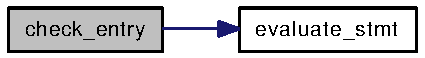
\includegraphics[width=120pt]{pf__administration_8h_754e9a8891128a285fc17132b5480a07_cgraph}
\end{center}
\end{figure}
\hypertarget{pf__administration_8h_2edf8cd83efaa23984150c5c7e62d628}{
\index{pf\_\-administration.h@{pf\_\-administration.h}!check\_\-entry\_\-string@{check\_\-entry\_\-string}}
\index{check\_\-entry\_\-string@{check\_\-entry\_\-string}!pf_administration.h@{pf\_\-administration.h}}
\subsubsection{\setlength{\rightskip}{0pt plus 5cm}int check\_\-entry\_\-string (char $\ast$ {\em number}, int {\em priority}, int {\em listflag})}}
\label{pf__administration_8h_2edf8cd83efaa23984150c5c7e62d628}


Checks if a number is on the blacklist/whitelist.

\begin{Desc}
\item[Parameters:]
\begin{description}
\item[{\em number}]The whole number with country code, area code and phone number. \item[{\em priority}]Gives the \hyperlink{structentry}{entry} a priority. 0 is standard. If the priority is higher the value will be also blocked/accepted if a higher priority is choosen. \item[{\em listflag}]A flag, which indicates if you would use the blacklist (BLACKLIST\_\-FLAG) or the whitelist (WHITELIST\_\-FLAG).\par
\end{description}
\end{Desc}
\begin{Desc}
\item[Returns:]If the number was found 1, otherwise 0. \end{Desc}


Definition at line 263 of file pf\_\-administration.c.

References BLACKLIST\_\-FLAG, DB\_\-FILE, ERR\_\-LOG, evaluate\_\-stmt\_\-string(), INFO\_\-LOG, MAX\_\-LINE\_\-LENGTH, STMT\_\-SIZE, TB\_\-AREACODE, TB\_\-COUNTRYCODE, TB\_\-NUMBER, TB\_\-PRIORITY, and WHITELIST\_\-FLAG.

Here is the call graph for this function:\nopagebreak
\begin{figure}[H]
\begin{center}
\leavevmode
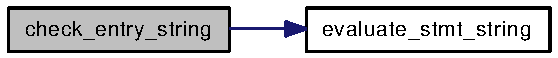
\includegraphics[width=152pt]{pf__administration_8h_2edf8cd83efaa23984150c5c7e62d628_cgraph}
\end{center}
\end{figure}
\hypertarget{pf__administration_8h_b6c4b54e76914072e8c0d06f9e450d33}{
\index{pf\_\-administration.h@{pf\_\-administration.h}!rm\_\-entry@{rm\_\-entry}}
\index{rm\_\-entry@{rm\_\-entry}!pf_administration.h@{pf\_\-administration.h}}
\subsubsection{\setlength{\rightskip}{0pt plus 5cm}int rm\_\-entry (int {\em country\_\-code}, int {\em area\_\-code}, unsigned long long {\em number}, int {\em listlfag})}}
\label{pf__administration_8h_b6c4b54e76914072e8c0d06f9e450d33}


Removes a number from the blacklist/whitelist.

\begin{Desc}
\item[Parameters:]
\begin{description}
\item[{\em country\_\-code}]The country code (for example 39 for Italy, 43 for Austria, and so one) \item[{\em area\_\-code}]The area code which indicates your mobile operator. \item[{\em number}]The number which will be deleted. \item[{\em listflag}]A flag, which indicates if you would use the blacklist (BLACKLIST\_\-FLAG) or the whitelist (WHITELIST\_\-FLAG).\par
\end{description}
\end{Desc}
\begin{Desc}
\item[Returns:]If all goes right 0, otherwise an error code. \end{Desc}


Definition at line 155 of file pf\_\-administration.c.

References DB\_\-FILE, ERR\_\-LOG, MAX\_\-LINE\_\-LENGTH, STMT\_\-SIZE, TB\_\-AREACODE, TB\_\-COUNTRYCODE, TB\_\-NUMBER, and WHITELIST\_\-FLAG.